\section{Introduction and Planning}
\subsection{Tiberius II}

This group's involvement in the Tiberius project began with Tiberius II - a four-wheeled fixed-axis variant of the robot. Comprised of an aluminium extrusion frame, four wheels and motors, a large battery pack and a number of sensors and other smaller components, this was a simplistic design from a mechanical standpoint.

\begin{figure}[!htb]
\begin{center}
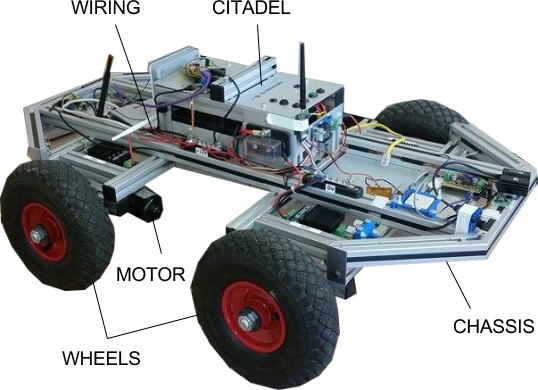
\includegraphics[width=10cm]{mechanical/figures_mech/mech_Tib_old_diagram.png}
\end{center}
\caption{Tiberius II}
\label{fig:mech_old}
\end{figure}

However, the group unanimously decided that there was room for improvement. The aluminium frame, while simple at first glance, was in fact over-designed; using far more material than required, making the robot unnecessarily heavy and components difficult to remove or replace.

In a similar fashion the wheel and motor system left much to be desired. While simple to use, the `tank style' steering caused excessive vibrations as the robot skidded around, and the jury-rigged motors (which were salvaged windscreen wiper motors from a car) flexed under the weight of the robot.

Clearly with so many changes it was likely that the entire structure of the robot would have to be changed. However, this opened up the opportunity to think about further mechanical features that would have been harder to implement while keeping the old robot intact. Drastic changes such as the addition of a steering system or shock absorbers to the frame would now be possible.

With so many possible changes in the pipeline it was decided that this project would culminate in an entirely new version of the Tiberius robot - Tiberius III.
\subsection{Aims and objectives}

With practically endless options for changing the design, the team settled on the below objectives:

\begin{enumerate}
	\item Motors
	\begin{itemize}
     	\item New motors
    	\item Velocity control
       	\item mbed control units
   	\end{itemize}
    
   	\item Wheel mounting
   	\begin{itemize}
     	\item Wheel unit
        \item Steering
        \item Suspension
   	\end{itemize}
    
	\item Chassis
   	\begin{itemize}
     	\item Reduced waste space
     	\item Refined mounts for sensors, batteries, and other equipment
     	\item Improved wiring standards
     	\item Finalised design iteration
   \end{itemize}
\end{enumerate}